\section{Latent Spaces and Embeddings}
\label{sec:LatentSpacesAndEmbeddings}

% ##############################################################################
\subsection{Learning Metric Embedding}
\label{ssec:LearningMetricEmbedding}

As Hermans~\etal{}~\cite{hermans2017triplet} describe, the goal of learning metric embedding is to learn a function $\func{f_\theta}{x}: \mathbb{R}^F \to \mathbb{R}^D$, which maps semantically similar points from the data manifold in $\mathbb{R}^F$ onto metrically close points in $\mathbb{R}^D$. Analogously, $\func{f_\theta}{\cdot}$ should map semantically different points in $\mathbb{R}^F$ onto metrically distant points in $\mathbb{R}^D$.

Suppose the use of this transformation for vehicle \gls{reid}. The corresponding embedding vector would be produced by a learned function that would map the images of vehicles into a latent space, where images of the same vehicle would be mapped closer together. Moreover, such mapping should be invariant to variations in lighting conditions, vehicle rotations, and many others. Among other things, embedding trained this way can be used to produce a feature vector for classification, one-shot learning tasks~\cite{koch2015siameseoneshot}, clustering~\cite{schroff2015facenet}, face recognition~\cite{parkhi2015deepface} and last, but not least, object \gls{reid}~\cite{kuma2019vehiclereid}.

% ##############################################################################
\subsection{Embedding Vector Similarity}
\label{ssec:EmbeddingVectorSimilarity}

There are various ways to evaluate the degree of similarity between embedding vectors. For simplicity as well as our purposes, we will discuss the two most common approaches, \ietext{}, Euclidean distance and cosine similarity.

Let $\vect{u}$ and $\vect{v}$ be arbitrary $D$-dimensional vectors representing our embedding vectors. The Euclidean distance between the vectord $\vect{u}$ and $\vect{v}$ is defined as
\begin{equation}
    \label{eq:EuclideanDistance}
    \euclnorm{\vect{u} - \vect{v}} =
    \sqrt{
        \sum_{i = 0}^{D} \rbrackets{\vect{u}_i - \vect{v}_i}^2
    },
\end{equation}
and the cosine similarity is defined as
\begin{equation}
    \label{eq:CosineSimilarity}
    \func{\cos \angle}{\vect{u}, \vect{v}} =
    \func{\cos}{\theta} =
    \frac{
        \vect{u} \cdot \vect{v}
    }{
        \euclnorm{\vect{u}} \euclnorm{\vect{v}}
    },
\end{equation}
where $\theta$ is the angle between the vectors $\vect{u}$ and $\vect{v}$.

% ##############################################################################
\subsection{Siamese and Triplet Networks}
\label{ssec:SiameseAndTripletNetworks}

% ------------------------------------------------------------------------------
\begin{figure}[t]
    \centering
    \begin{subfigure}[b]{0.49\textwidth}
        \centering
        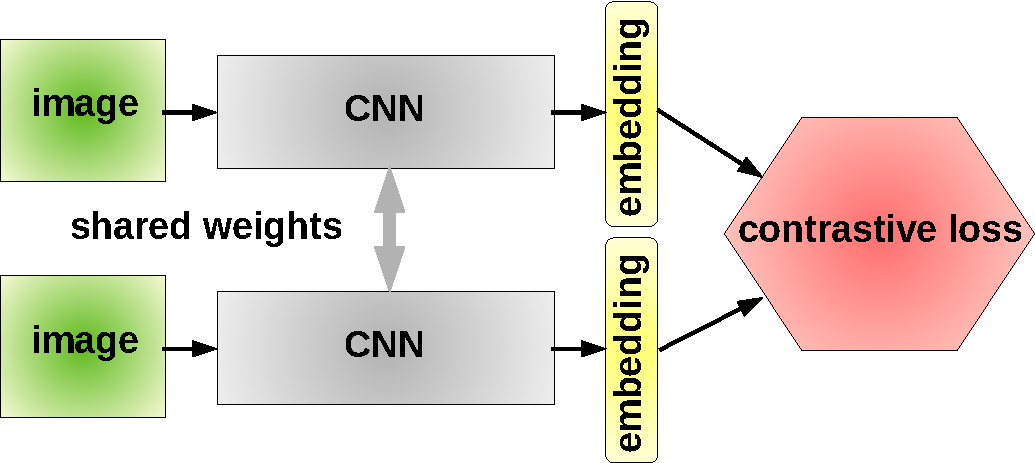
\includegraphics[width=\textwidth]{figures/theoretical_foundations/siamese_architecture.pdf}
        \caption[]{}
    \end{subfigure}
    \hfill
    \begin{subfigure}[b]{0.49\textwidth}
        \centering
        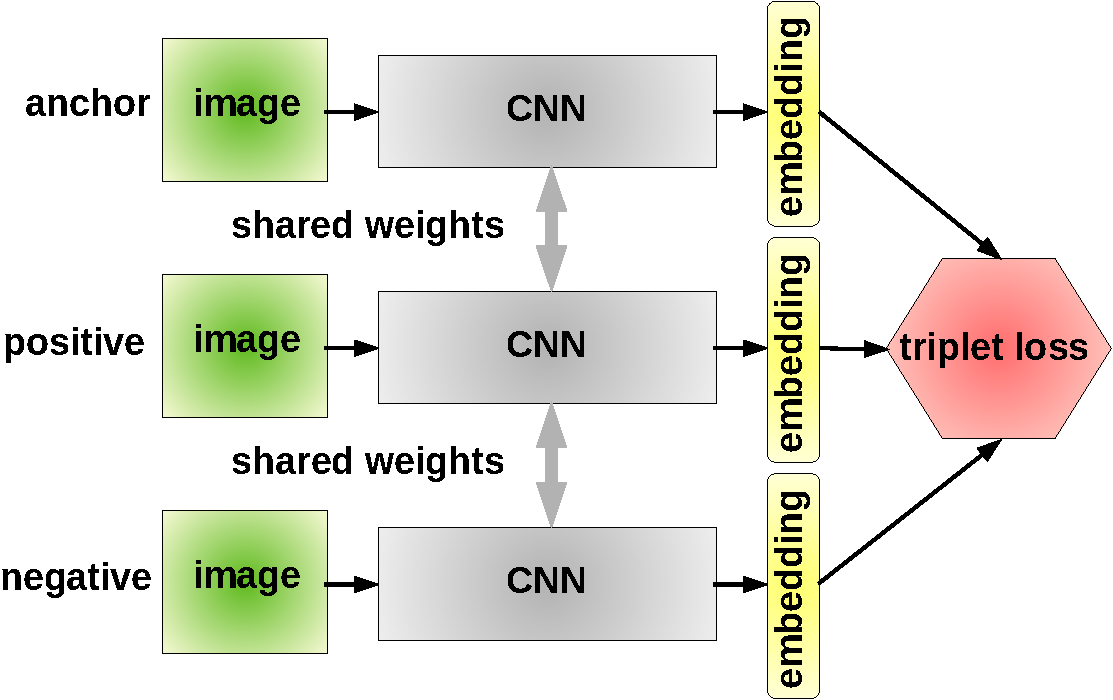
\includegraphics[width=\textwidth]{figures/theoretical_foundations/triplet_architecture.pdf}
        \caption[]{}
    \end{subfigure}
    \caption[Contrastive and triplet loss]{Comparison of the Siamese \imgpartdesc{a} and the triplet \imgpartdesc{b} network architectures. The concept of weight sharing implies that only one set of model weights is trained.}
    \label{fig:SiameseAndTripletArchitectures}
\end{figure}
% ------------------------------------------------------------------------------

For the upcoming discussion, let $\func{D}{x, y}: \mathbb{R}^D \times \mathbb{R}^D \to \mathbb{R}$ be a metric function measuring distances in the embedding space. Without a loss of generality, we resort to use of the Euclidean distance ($L_2$ norm), so $\func{D}{x, y} = \euclnorm{x - y}$.

\subsubsection{Contrastive Loss}

Consider a sample $\rbrackets{x_0, x_1, y}$, where $x_0$ and $x_1$ represent the input, and the label $y = 1$ if $x_0$ and $x_1$ belong to the same category, otherwise $y = 0$. $\func{D}{\cdot}$ is the previously defined metric function, and $\alpha$ is the margin representing the minimum distance in the metric space to separate positive from negative samples. Then the contrastive function for any sample is defined as~\cite{hadsell2006dimreduction}
\begin{equation}
    \label{eq:ContrastiveLoss}
    \func{\mathcal{L}_{contr}}{\theta} =
    \frac{1}{2}y
    {\func{D}{\func{f_\theta}{x_0}, \func{f_\theta}{x_1}}}^2 +
    \frac{1}{2}
    \rbrackets{1 - y} {\rbrackets{
            \sbrackets{\alpha - \func{D}{\func{f_\theta}{x_0}, \func{f_\theta}{x_1}}}_{+}}}^2.
\end{equation}
The two inputs $x_0$ and $x_1$ are fed to the shared model at the same time. The output is then evaluated by the contrastive loss function (\figtext{}~\ref{fig:SiameseAndTripletArchitectures} \imgpartdesc{a}). Positive samples should have a small distance between each other as measured by the $\func{D}{\cdot}$ to decrease the loss towards $0$. Conversely, negative samples should have a distance beyond the threshold $\alpha$.

\subsubsection{Triplet Loss}

Apart from the contrastive loss, this time three samples are required to compute the loss. The rationale is to supply additional context when forming the metric space. Siamese networks are usually implemented using shared model weights, but there are better approaches when the triplet loss is used. Conceptually speaking, the model could be implemented as shown in \figtext{}~\ref{fig:SiameseAndTripletArchitectures} \imgpartdesc{b}. However, as we will discuss later, triplet mining strategies are required for the triplet loss to work properly. The model can be thus simplified from an architectural point of view at the cost of moving the complexity to the computation of the loss function.

Let $N$ be the number of all possible valid triplets $\rbrackets{x_a^i, x_p^i, x_n^i}$ for a given dataset. For any $i$-th triplet, let $x_a^i$ be the \emph{anchor} for a specific object (person, vehicle, etc.) with label $\func{y}{x_a^i}$, $x_p^i$ be the positive sample of the same object with label $\func{y}{x_p^i}$, such that $x_a^i \neq x_p^i \land \func{y}{x_a^i} = \func{y}{x_p^i}$, and let $x_n^i$ with label $\func{y}{x_n^i}$ be a sample of any other object, satisfying $\func{y}{x_a^i} \neq \func{y}{x_n^i}$, $\forall i = 1, \dots, N$. Let $\alpha$ be the margin value that is enforced between positive and negative pairs. Then, we want the relationship
\begin{equation}
    \label{eq:TripletDistanceConstraint}
    \func{D}{\func{f_\theta}{x_a^i}, \func{f_\theta}{x_p^i}} + \alpha < \func{D}{\func{f_\theta}{x_a^i}, \func{f_\theta}{x_n^i}}, \forall i = 1, \dots, N,
\end{equation}
to hold true. The triplet loss function is therefore defined as
\begin{equation}
    \label{eq:TripletLoss}
    \func{\mathcal{L}_{triplet}}{\theta} =
    \sum_{i = 1}^{N}
    {\sbrackets{
        \alpha +
        \func{D}{\func{f_\theta}{x_a^i}, \func{f_\theta}{x_p^i}} -
        \func{D}{\func{f_\theta}{x_a^i}, \func{f_\theta}{x_n^i}}
    }}_+.
\end{equation}
During the training using the triplet loss, the model should learn to push negative samples further away from the positive samples, ideally exceeding the margin $\alpha$. Assuming a situation when the negative sample is mapped closer than a positive sample, the training should result in the desired situation of bringing the positive sample closer while pushing the negative one further (\figtext{}~\ref{fig:TripletLossLearningProcess}).

% ------------------------------------------------------------------------------
\begin{figure}[t]
    \centerline{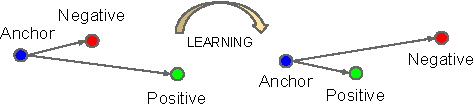
\includegraphics[width=0.6\linewidth]{figures/theoretical_foundations/triplet_loss_learning_process.pdf}}
    \caption[Triplet loss learning]{The objective is to learn embeddings such that the anchor is closer to the positive example than it is to the negative example by some specified margin value. \externalsrc{\cite{schroff2015facenet}}}
    \label{fig:TripletLossLearningProcess}
\end{figure}
% ------------------------------------------------------------------------------

% ##############################################################################
\subsection{Triplet Mining Strategies}
\label{ssec:TripletMiningStrategies}

Contrastive (\eqtext{}~\ref{eq:ContrastiveLoss}) and triplet (\eqtext{}~\ref{eq:TripletLoss}) loss functions play an important role in training an embedding model. However, the way that pairs or triplets are selected is crucial, and as Hermans~\etal{}~\cite{hermans2017triplet} and Manmatha~\etal{}~\cite{manmatha2017samplingmatters} showed, it may significantly influence the training. Moreover, as the dataset gets larger, then the number of possible triplets grows cubically, rendering the use of all of them impractical. The majority of those triplets would be so-called \emph{easy triplets}, thus hindering the learning process. To paraphrase the analogy from~\cite{hermans2017triplet}, showing the model that people with different clothes are not the same person after a certain point does not bring any new information. On the other hand, explicitly \emph{mining} images of similar-looking yet different people with the same clothes (\emph{hard negatives}) or of the same person with dramatically different poses (\emph{hard positives}) vastly contributes to an understanding of the notion of the \emph{same person}. As suggested, there are different kinds of triplets which are defined in \tabletext{}~\ref{tab:TripletCategoriesDefinitions}, using a general $\rbrackets{x_a^i, x_p^i, x_n^i}$ triplet for clarity. We encourage the reader to observe \figtext{}~\ref{fig:PositiveAndNegativeTripletsCategories}, too.

\begin{table}[t]
    \centering

    \begin{tabular}{cc}
        \toprule
        \tblcolname{triplet} & \tblcolname{constraint}                                                                                                                                            \\

        \midrule
        \emph{easy}          &
        $\func{D}{\func{f_\theta}{x_a^i}, \func{f_\theta}{x_p^i}} + \alpha < \func{D}{\func{f_\theta}{x_a^i}, \func{f_\theta}{x_n^i}}$                                                            \\

        \emph{semi-hard}     &
        $\func{D}{\func{f_\theta}{x_a^i}, \func{f_\theta}{x_p^i}} < \func{D}{\func{f_\theta}{x_a^i}, \func{f_\theta}{x_n^i}} < \func{D}{\func{f_\theta}{x_a^i}, \func{f_\theta}{x_p^i}} + \alpha$ \\

        \emph{hard}          & $\func{D}{\func{f_\theta}{x_a^i}, \func{f_\theta}{x_n^i}} < \func{D}{\func{f_\theta}{x_a^i}, \func{f_\theta}{x_p^i}}$                                              \\
        \bottomrule
    \end{tabular}

    \caption[Triplet categories.]{Definitions of various categories of triplets (regardless whether it is positive or negative) as imposed by their distance relationship.}
    \label{tab:TripletCategoriesDefinitions}
\end{table}

% ------------------------------------------------------------------------------
\begin{figure}[t]
    \centering
    \begin{subfigure}[b]{0.35\textwidth}
        \centering
        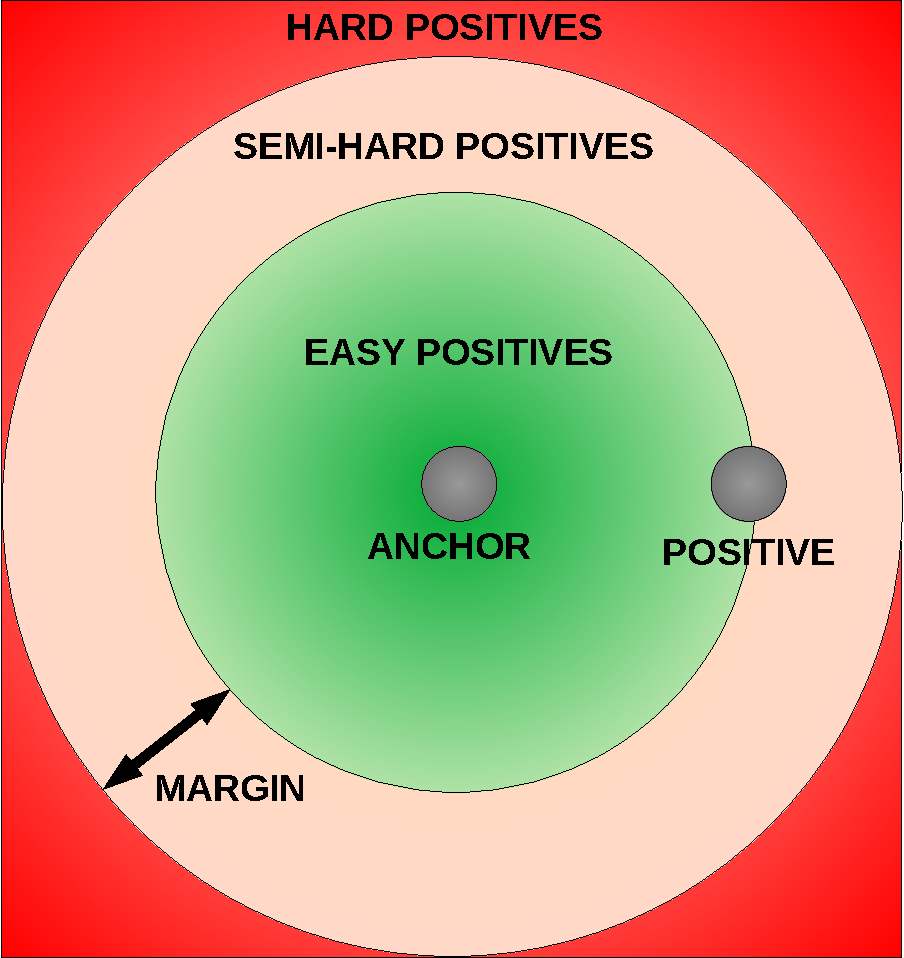
\includegraphics[width=\textwidth]{figures/theoretical_foundations/triplet_positives_categories.pdf}
        \caption[]{}
    \end{subfigure}
    \hfill
    \begin{subfigure}[b]{0.35\textwidth}
        \centering
        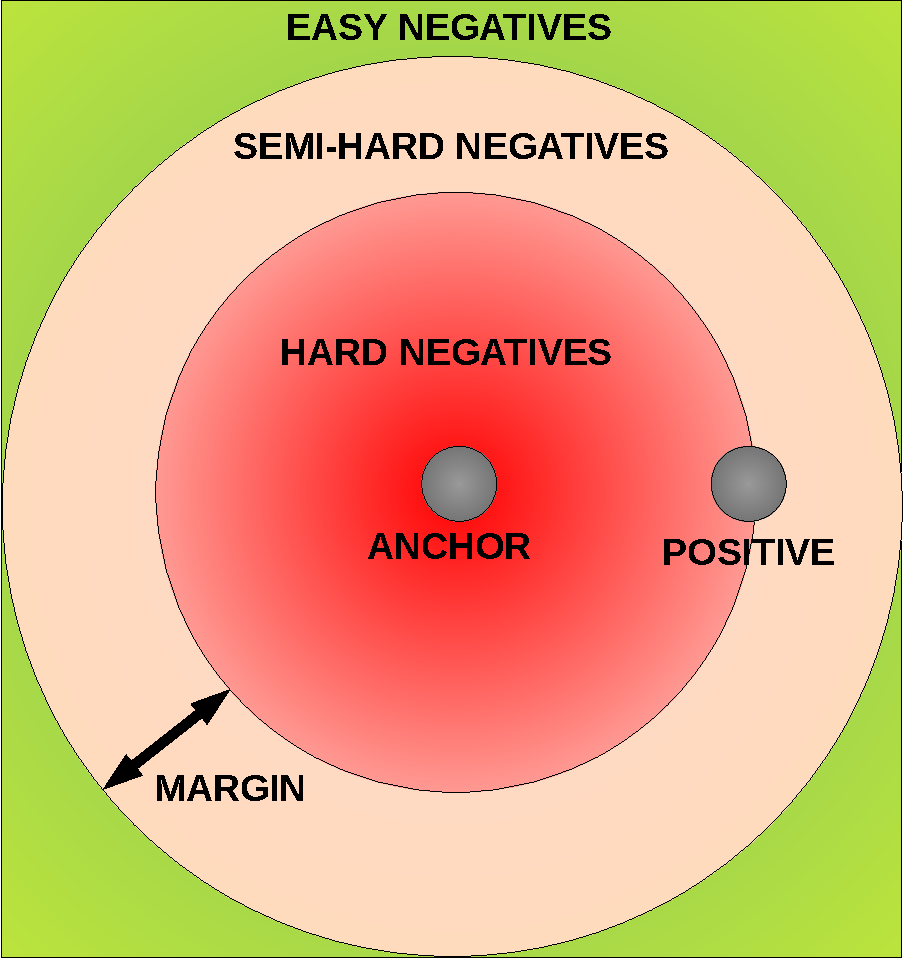
\includegraphics[width=\textwidth]{figures/theoretical_foundations/triplet_negatives_categories.pdf}
        \caption[]{}
    \end{subfigure}
    \caption[Triplet loss categories visualization.]{Given a fixed anchor $x_a^i$ and positive sample $x_p^i$ as well as some positive margin value $\alpha$, we discriminate between three different types of categories in terms of their level of \emph{difficulty}. These categories vary in relation to positive \imgpartdesc{a} or negative \imgpartdesc{b} perspective.}
    \label{fig:PositiveAndNegativeTripletsCategories}
\end{figure}
% ------------------------------------------------------------------------------

In order to attain an effective convergence during the training, it is necessary to select triplets that violate the triplet constraint in \eqtext{}~\ref{eq:TripletDistanceConstraint}. This means that given $x_a^i$, the goal is to select a \emph{hard positive} $x_p^i$ given by $\argmax_{x_p^i}\cbrackets{\func{D}{\func{f_\theta}{x_a^i}, \func{f_\theta}{x_p^i}}}$ and a \emph{hard negative} $x_n^i$ as a result of $\argmin_{x_n^i}\cbrackets{\func{D}{\func{f_\theta}{x_a^i}, \func{f_\theta}{x_n^i}}}$. Admittedly, it is often infeasible to compute the $\argmin\cbrackets{\cdot}$ and $\argmax\cbrackets{\cdot}$ over the entire training set. In this regard, there are two possible approaches to tackle this problem, either by selecting these hard triplets online or doing it offline~\cite{schroff2015facenet}.

\subsubsection{Offline Triplet Mining}

Given a training set, the task is to produce reasonable triplets off-line, for instance, at the epoch beginning. First, a list of $N$ different valid triplets is randomly generated, then separated into $\lfloor \nicefrac{N}{B} \rfloor$ batches of $B$ triplets, followed by computation of $3N$ embeddings using the most recent model checkpoint. Then, hard or semi-hard triplets may be selected. Since this strategy has been shown on multiple occasions~\cite{schroff2015facenet, hermans2017triplet, kuma2019vehiclereid} as an inferior choice compared to the online triplet mining, we will not discuss this approach further.

\subsubsection{Online Triplet Mining}

Online mining is performed by selecting the hard positive/negative exemplars from within a mini-batch (\figtext{}~\ref{fig:TripletArchitectureOnlineMining}). A condition that a minimum number of exemplars for any identity is present in each mini-batch has to be met. For example, Schroff~\etal{}~\cite{schroff2015facenet} used $40$ different images of a single person (an identity) per mini-batch. Let $P$ be the number of different objects/identities (\egtext{}, people, vehicles) and $K$ be the number of different images for a concrete identity (\egtext{} different views of the same vehicle). There are two prominent approaches to online mining: \emph{batch all} and \emph{batch hard}.

% ------------------------------------------------------------------------------
\begin{figure}[t]
    \centerline{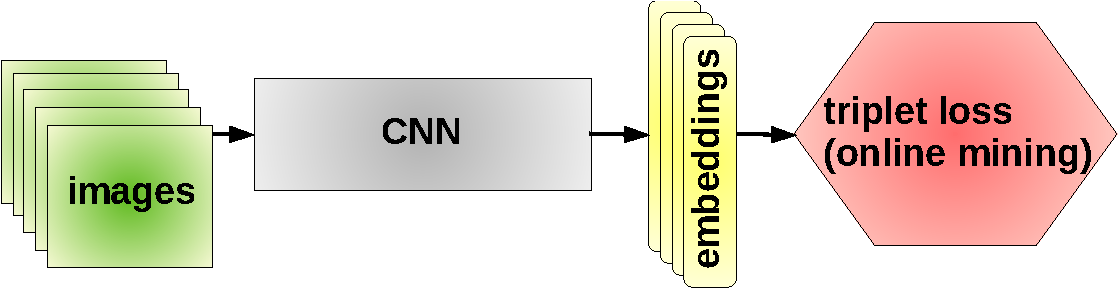
\includegraphics[width=0.5\linewidth]{figures/theoretical_foundations/triplet_architecture_online_mining.pdf}}
    \caption[Triplet loss online mining architecture]{The architecture of a triplet network where an online triplet loss function is used for training. In this architecture, no weight sharing is required as the triplet selection happens \emph{online} solely in the loss function.}
    \label{fig:TripletArchitectureOnlineMining}
\end{figure}
% ------------------------------------------------------------------------------

\subsubsection{Online Triplet Mining: Batch All}

This strategy aims for selecting all valid triplets and averaging the loss only on the hard and semi-hard triplets. Easy triplets, \ietext{}, those for which the loss function equals $0$, are not taken into account. The reason is that averaging on them would result in a very small loss, since they would usually vastly outnumber the set of hard triplets~\cite{hermans2017triplet}. This approach produces a total of $PK \rbrackets{K - 1} \rbrackets{PK - K}$ triplets ($PK$ anchors, $K - 1$ positives per anchors, $PK - K$ negatives) incorporated in the loss function as
\begin{equation}
    \label{eq:BatchAllLossFunction}
    \begin{aligned}
        \func{\mathcal{L}_{batchall}}{\theta} =
        \sum_{i = 1}^P
        \sum_{a = 1}^K
        \sum_{\substack{p = 1 \\p \neq a}}^K
        \sum_{\substack{j = 1 \\j \neq i}}^P
        \sum_{n = 1}^K
        \Bigg[
         & \alpha +           \\
         & \func{D}{
            \func{f_\theta}{x_a^i},
            \func{f_\theta}{x_p^i}
        } -                   \\
         & \func{D}{
            \func{f_\theta}{x_a^i},
            \func{f_\theta}{x_n^j}
        }
        {\Bigg]}_{+}.
    \end{aligned}
\end{equation}

\subsubsection{Online Triplet Mining: Batch Hard}

In this strategy, the goal is to find the hardest positive and hardest negative for each anchor. The total number of triplets is $PK$. The selected triplets are the hardest among the given batch and can be considered moderate since they are the hardest within a small subset of the data. Therefore, the mining can be formulated as
\begin{equation}
    \label{eq:BatchHardMining}
    \begin{aligned}
        \func{\mathcal{L}_{batchhard}}{\theta} =
        \sum_{i = 1}^P
        \sum_{a = 1}^K
        \Bigg[
         & \alpha +                            \\
         & \underset{p = 1, \dots, K} {\max}
        \cbrackets{
            \func{D}{
                \func{f_\theta}{x_a^i},
                \func{f_\theta}{x_p^i}
            }
        } -                                    \\
         & \underset{\substack{j = 1, \dots, P \\n = 1, \dots, K\\j \neq i}} {\min}
        \cbrackets{
            \func{D}{
                \func{f_\theta}{x_a^i},
                \func{f_\theta}{x_n^j}
            }
        }
        {\Bigg]}_{+}
    \end{aligned}
\end{equation}
